\mode*
\section{C Concepts}

\begin{frame}[fragile]{The \texttt{\#include} Instruction}
  \begin{center}
    \includegraphics[scale=1.5]{include-c}\tikzmark{inc}
  \end{center}
\begin{description}
\item[Header files:] for keeping \emph{definitions} and \emph{function prototypes}. E.g.
  \begin{itemize}
  \item \mintinline{c}{#define SQR(x) ((x) * (x))}
  \item \mintinline{c}{ssize_t read(int fildes, void *buf, size_t nbyte);}
  \end{itemize}
\item[Stan\tikzmark{std}dard header files:] define data structures, macros, and function
  prototypes used by library routines, e.g. \texttt{printf()}.
  \begin{itemize}
  \item[\$] \texttt{ls /usr/include}
  \end{itemize}
\item[Loc\tikzmark{local}al include files:] self-defined data structures, macros, and
  function prototypes.
\end{description}
\begin{itemize}
\item[\$] \texttt{gcc -E hello.c}
\end{itemize}
\begin{tikzpicture}[remember picture,overlay,->,blue,ultra thick,opacity=.1]
  \draw ($(pic cs:std)+(0,1ex)$) to[bend left=25] ($(pic cs:inc)+(-2.8,.8)$);
  \draw ($(pic cs:local)+(0,1ex)$) to[bend left=20] ($(pic cs:inc)+(-2.8,.2)$);
\end{tikzpicture}
\end{frame}

\begin{frame}{The \texttt{\#define} Instruction}
  \begin{block}{Always put \alert{\{ \}} around all multi-statement macros!}
    \begin{center}
      \mode<beamer>{
        \includegraphics[width=.8\textwidth]{die-wrong-c}\tikzmark{die-wrong}
        \begin{tikzpicture}[remember picture,overlay,opacity=.3]
          \node (wrong) [scale=5] at ($(pic cs:die-wrong)+(0,3)$) {\RedCross};
        \end{tikzpicture}
      }%
      \mode<article>{
        \includegraphics[width=.4\textwidth]{die-wrong-c}\tikzmark{die-wronga}
        \begin{tikzpicture}[remember picture,overlay,opacity=.3]
          \node (wrong) [scale=5] at ($(pic cs:die-wronga)+(0,2)$) {\RedCross};
        \end{tikzpicture}
      }
    \end{center}
  \end{block}
  \begin{block}{}
    \begin{center}
      \mode<beamer>{ \includegraphics[width=.8\textwidth]{die-right-c}\tikzmark{die-right} }%
      \mode<article>{ \includegraphics[width=.4\textwidth]{die-right-c}\tikzmark{die-right} }
    \end{center}
  \end{block}
  \begin{description}
  \item[Why?] \texttt{gcc -E}
  \end{description}
  \begin{tikzpicture}[remember picture,overlay,opacity=.3]
    \node (right) [scale=5,green] at (pic cs:die-right) {\Checked};
  \end{tikzpicture}
\end{frame}

\begin{frame}[fragile=singleslide]
  \begin{block}{Always put \alert{( )} around the parameters of a macro!}
    \begin{center}
      \mode<beamer>{
        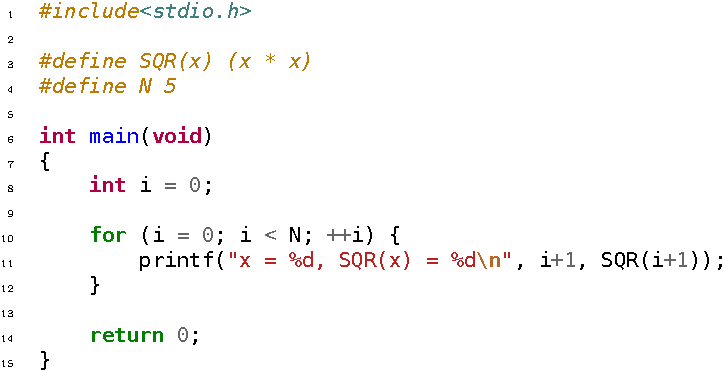
\includegraphics[width=\textwidth]{sqr-wrong-c}\tikzmark{sqr-wrong}
        \begin{tikzpicture}[remember picture,overlay,opacity=.3]
          \node [scale=5] at ($(pic cs:sqr-wrong)+(-6,4.5)$) {\RedCross};
        \end{tikzpicture}
      }%
      \mode<article>{
        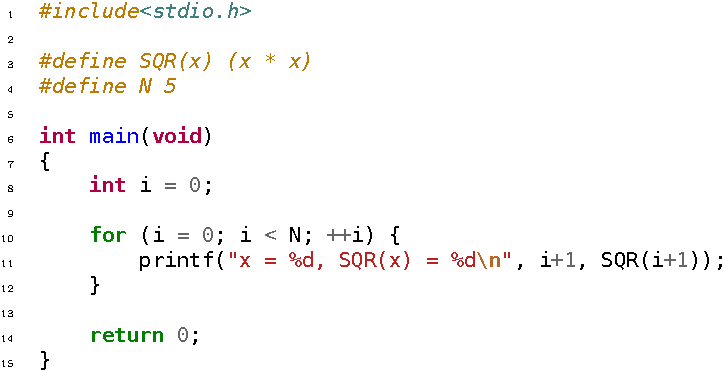
\includegraphics[width=.5\textwidth]{sqr-wrong-c}\tikzmark{sqr-wronga}
        \begin{tikzpicture}[remember picture,overlay,opacity=.3]
          \node [scale=5] at ($(pic cs:sqr-wronga)+(-4,3.2)$) {\RedCross};
        \end{tikzpicture}
      }
    \end{center}
  \end{block}
  \begin{itemize}
  \item[\Checked] \mintinline{c}{#define SQR(x) ((x) * (x))}
  \item[\$] \texttt{gcc -E}
  \end{itemize}
\end{frame}

\begin{frame}{Bitwise Operations}
  \begin{center}
    \mode<beamer>{ \includegraphics[width=\textwidth]{bitwise-c} }%
    \mode<article>{\cfile{../src/bitwise.c}}
  \end{center}
\end{frame}

\begin{frame}{Pointers}
  \begin{center}
    \mode<beamer>{ \includegraphics[width=.9\textwidth]{ptr1-code-c} }%
    \mode<article>{\cfile{../src/ptr1-code.c}}
  \end{center}
  \begin{center}
    \mode<beamer>{ \includegraphics[width=\textwidth]{ptr1} }%
    \mode<article>{ \includegraphics[width=.6\textwidth]{ptr1} }
  \end{center}
\end{frame}

\begin{frame}{Pointer Operators}
  \begin{itemize}
  \item[\&] returns the \alert{address} of a thing
  \item[{\dejavu ✶}] return the \alert{object (thing)} to which a pointer points at
  \end{itemize}
  \begin{block}{\texttt{int thing; int *thing\_ptr;}}
    \begin{center}
      \begin{tabular}{rl}\hline
        \thead{C Code}&\thead{Description}\\\hline
        \texttt{thing}& the variable named `thing'\\
        \texttt{\&thing}& address of `thing' (a pointer)\\
        \texttt{*thing}& \RedCross{}\\
        \texttt{thing\_ptr}& pointer to an int\\
        \texttt{*thing\_ptr}& the int variable at the address \texttt{thing\_ptr} points
                              to\\
        \texttt{\&thing\_ptr}& odd, a pointer to a pointer\\\hline
      \end{tabular}
    \end{center}
  \end{block}
\end{frame}

\begin{frame}
  \begin{block}{Example}
    \begin{center}
      \mode<beamer>{ \includegraphics[width=.9\textwidth]{ptr2-code-c} }%
      \mode<article>{\cfile{../src/ptr2-code.c}}
    \end{center}
  \end{block}
  \begin{center}
    \mode<beamer>{ \includegraphics[width=.8\textwidth]{ptr2} }%
    \mode<article>{ \includegraphics[width=.4\textwidth]{ptr2} }
  \end{center}
\end{frame}

\begin{frame}
  \begin{block}{Invalid operation}
    \begin{center}
      \mode<beamer>{ 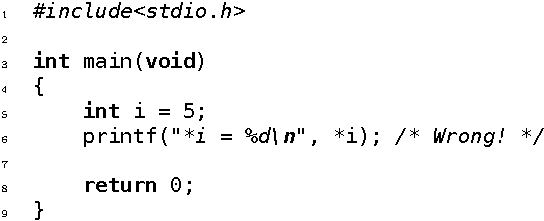
\includegraphics[width=.7\textwidth]{ptr2-wrong1-c} }%
      \mode<article>{\cfile{../src/ptr2-wrong1.c}}
    \end{center}
    \mode<article>{
      This is trying to treat the value of \texttt{i} as an memory address. But the memory
      address \texttt{5} is not accessible by this program.
    }
  \end{block}
  \begin{block}{Invalid memory access}
    \begin{center}
      \mode<beamer>{ 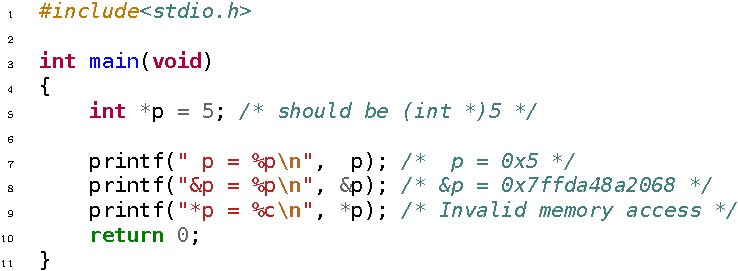
\includegraphics[width=.8\textwidth]{ptr2-wrong2-c} }%
      \mode<article>{ 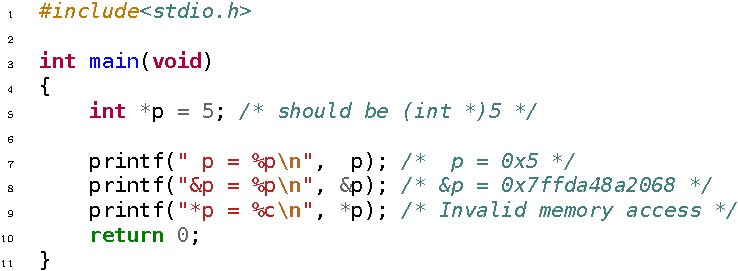
\includegraphics[width=.6\textwidth]{ptr2-wrong2-c} }
    \end{center}
    \mode<article>{This is trying to treat the value of \texttt{p} as an memory
      address. But the memory address \texttt{5} is not accessible by this program.}
  \end{block}
\end{frame}

\begin{frame}{Call by Value}
  \begin{center}
    \mode<beamer>{
      \includegraphics[width=.6\textwidth]{ptr4-wrong-c}\tikzmark{ptr4wrong}
      \pause
      \begin{tikzpicture}[remember picture,overlay]
        \node at ($(pic cs:ptr4wrong)+(1,2)$) [opacity=.4,scale=7] {\RedCross};
      \end{tikzpicture}}%    
    \mode<article>{
      \includegraphics[width=.3\textwidth]{ptr4-wrong-c}\tikzmark{ptr4wronga}
      \begin{tikzpicture}[remember picture,overlay]
        \node at ($(pic cs:ptr4wronga)+(1,2)$) [opacity=.4,scale=7] {\RedCross};
      \end{tikzpicture}}    
  \end{center}
  \begin{description}
  \item[Call by value:] only the \alert{value} of `\texttt{count}' is handed to the
    function \texttt{inc\_count()}
  \end{description}
\end{frame}

\begin{frame}
  \begin{block}{Solution 1: return}
    \begin{center}
      \mode<beamer>{
        \includegraphics[width=.7\textwidth]{ptr4-ok-c}
        \begin{tikzpicture}[remember picture,overlay]
          \node at ($(pic cs:ptr4ok)+(0,2)$) [opacity=.4,scale=10,red] {\Checked};
        \end{tikzpicture}}%
      \mode<article>{
        \includegraphics[width=.4\textwidth]{ptr4-ok-c}\tikzmark{ptr4oka}
        \begin{tikzpicture}[remember picture,overlay]
          \node at ($(pic cs:ptr4oka)+(0,2)$) [opacity=.4,scale=10,red] {\Checked};
        \end{tikzpicture}
        \begin{enumerate}
        \item read the \emph{value} of \texttt{count}, and pass it to \texttt{inc\_count()};
        \item \texttt{inc\_count()} uses the \emph{value} of \texttt{count} to do the
          calculations;
        \item return the result to \texttt{main()}.
        \end{enumerate}
      }
    \end{center}
  \end{block}
\end{frame}

\begin{frame}{Pointers as Function Arguments}
  \begin{block}{Solution 2: Call by reference}
    \begin{center}
      \mode<beamer>{
        \includegraphics[width=.6\textwidth]{ptr4-c}
        \begin{tikzpicture}[remember picture,overlay]
          \node at ($(pic cs:ptr4)+(0,2)$) [opacity=.4,scale=10,red] {\Checked};
        \end{tikzpicture}}%
      \mode<article>{
        \includegraphics[width=.3\textwidth]{ptr4-c}\tikzmark{ptr4a}
        \begin{tikzpicture}[remember picture,overlay]
          \node at ($(pic cs:ptr4a)+(0,2)$) [opacity=.4,scale=10,red] {\Checked};
        \end{tikzpicture}
        \begin{enumerate}
        \item pass the address of \texttt{count} to \texttt{inc\_count()};
        \item \texttt{inc\_count()} operates directly on \texttt{count}.
        \end{enumerate}
        This is more efficient than solution 1 (Imagining you are operating on a large
        data structure rather than an \texttt{int}). 
      }
    \end{center}
  \end{block}    
\end{frame}

\begin{frame}[fragile]{\texttt{const} Pointers}
\begin{ccode}
const char *a_ptr = "Test";
char *const a_ptr = "Test";
const char *const a_ptr = "Test";
\end{ccode}
  \begin{enumerate}
  \item The da\tikzmark{data1}ta cannot change, but the poin\tikzmark{ptr1}ter can
  \item The point\tikzmark{ptr2}er cannot change, but the \tikzmark{data2}data it points to can
  \item Neither can change
  \end{enumerate}
  \mode<beamer>{
  \begin{tikzpicture}[remember picture,overlay,->,blue,ultra thick, opacity=.1]
  \draw ($(pic cs:data1)+(0,1ex)$) to[bend left=25] ($(current page.center)+(-1.5,1.8)$);
  \draw ($(pic cs:ptr1)+(0,1ex)$) .. controls +(1,1.5) and +(1.5,1.2) .. ($(current page.center)+(-2.3,1.9)$);
  \draw ($(pic cs:data2)+(0,1ex)$) to ($(current page.center)+(-.8,1.3)$);
  \draw ($(pic cs:ptr2)+(0,1ex)$) to ($(current page.center)+(-2.4,1.3)$);
\end{tikzpicture}}
\end{frame}

\mode<all>
%%% Local Variables:
%%% mode: latex
%%% TeX-master: "c-b"
%%% End:
